% ============================================================================
% AFOSR FY2027 Young Investigator Program (YIP) --- White Paper, A.2.c version
% NOFO FA955026S0003; due 2026-10-09, 11:59 PM ET, via the AFOSR Qualtrics
% portal: https://afosr.gov1.qualtrics.com/jfe/form/SV_eKuTqm9qezoDYep
%
% Research discipline area: Dynamic Data and Information Processing
% (BAA FA955026S0001 Amdt 0001, Sec. A.2.c; Dr. Erik Blasch, AFOSR/RESA,
% D2IP@us.af.mil). The A.3.a (Sayir) version is afosr-yip-white-paper.tex.
%
% Demonstration system: aluminum alloys. The induction-melting module of the
% lab's atomizer covers aluminum but not refractory alloys or Ni superalloys,
% which need the plasma module (not requested here).
% The atomizer makes four compositions per week. LPBF builds are bought as a
% fee-for-service from a University of Utah user facility at $800 per build
% (Sterling, PR #90, 2026-10-10). The BOFN simulation in Section 5 charged
% $2,500 per build; its per-step costs are rough estimates of total cost
% (time, materials, supplies), so Section 5 says so instead of quoting $800.
%
% Format rules, required content, and the 1.5-line spacing definition are the
% same as in afosr-yip-white-paper.tex (NOFO pp. 21-22).
%
% Prose checked with cringe-filter (https://github.com/sgbaird/cringe-filter):
%   cringe-filter lint  -c proposal afosr-yip-white-paper-a2c.tex
%   cringe-filter score -c proposal afosr-yip-white-paper-a2c.tex
%
% Build:  make a2c
% ============================================================================

% NOFO p. 21: a PI who submits more than one white paper must acknowledge the
% others on each. Only this one is being submitted (Sterling, PR #90,
% 2026-10-10), so the cover has no "Other white papers" line.

\documentclass[12pt,letterpaper]{article}

% --- Page geometry (NOFO: 8.5 x 11 in, 1 in margins) ---
\usepackage[margin=1in]{geometry}

% --- Fonts (NOFO: Times New Roman or Garamond, 12 pt) ---
\usepackage{iftex}
\ifPDFTeX
  \usepackage[T1]{fontenc}
  \usepackage[utf8]{inputenc}
  \usepackage{mathptmx}  % Times clone for pdfLaTeX builds
\else
  \usepackage{fontspec}
  \IfFontExistsTF{Times New Roman}
    {\setmainfont{Times New Roman}}
    {\setmainfont{TeX Gyre Termes}}
\fi
\usepackage{microtype}

% --- Spacing (NOFO: 1.5-line spacing) ---
\usepackage{setspace}
\setstretch{1.43}  % 14.5 pt x 1.43 = 20.7 pt = Word "1.5 lines" for TNR 12 pt
\setlength{\parindent}{0pt}
\setlength{\parskip}{3pt plus 2pt minus 1pt}
\setlength{\textfloatsep}{12pt plus 2pt minus 2pt}
\setlength{\floatsep}{8pt plus 2pt minus 2pt}

% --- Figures, tables, CV ---
\usepackage{graphicx}
\usepackage{tikz}
\usetikzlibrary{positioning,arrows.meta,fit}
\usepackage{array}
\usepackage{pdfpages}
\usepackage{wrapfig}
\usepackage[font={normalsize,stretch=1.43},labelfont=bf,labelsep=period,
  skip=4pt]{caption}

% --- References and links ---
\usepackage[
  colorlinks=true,
  linkcolor=blue!70!black,
  citecolor=blue!70!black,
  urlcolor=blue!70!black
]{hyperref}

% --- Section headings (12 pt, compact) ---
\usepackage{titlesec}
\titleformat{\section}{\normalfont\normalsize\bfseries}{\thesection.}{0.5em}{}
\titlespacing*{\section}{0pt}{8pt plus 2pt minus 2pt}{0pt}
\titleformat{\subsection}[runin]{\normalfont\normalsize\bfseries}{}{0pt}{}[.]
\titlespacing*{\subsection}{0pt}{6pt plus 2pt minus 1pt}{0.5em}

% --- Page numbers only, in the bottom margin ---
\pagestyle{plain}

\newcommand{\degC}{\textdegree{}C}
\hyphenation{re-POW-DER AMA-ZE-MET}

\begin{document}

% ===========================================================================
% Cover page (excluded from the 5-page limit)
% ===========================================================================
\begin{titlepage}
\begin{center}
{\Large\bfseries Dynamic Data-Driven Selection of Experiments\\
for Laser-Printed Aluminum Alloys\par}
\vspace{18pt}
White paper\\
Air Force Office of Scientific Research (AFOSR)\\
FY2027 Air Force Young Investigator Program (YIP)
\end{center}
\vspace{18pt}
\begin{tabular}{@{}>{\bfseries}p{1.9in}>{\raggedright\arraybackslash}p{4.4in}@{}}
NOFO number & FA955026S0003 \\
Research discipline area & Dynamic Data and Information Processing
  (AFOSR BAA FA955026S0001, Section A.2.c). Program Officer: Dr.~Erik
  Blasch, AFOSR/RESA \\
Principal investigator & Sterling G.\ Baird, Ph.D. \\
Position & Assistant Professor, Department of Mechanical Engineering,
  Brigham Young University (BYU), 350 EB, Provo, UT 84602 \\
Telephone & (801) 422-5344 \\
Email & \href{mailto:sterling.baird@byu.edu}{sterling.baird@byu.edu} \\
Doctorate & Ph.D., Materials Science and Engineering, University of Utah,
  August 2023 \\
Period and cost & 36 months, up to \$150,000 per year (\$450,000 total) \\
\end{tabular}
\end{titlepage}

\setcounter{page}{1}

% ===========================================================================
% White paper body (5-page limit)
% ===========================================================================
\section{Proposed research and scientific issues}

Developing a new alloy for laser powder bed fusion (LPBF) runs through a chain
of steps: a thermodynamic calculation, powder production, single laser tracks
and small printed cubes, microscopy, and finally tensile tests. Their costs
differ greatly: a thermodynamic calculation takes minutes, a set of laser
tracks hours, and a tensile test on machined specimens days. Experimental
campaigns often send each candidate through the whole chain, spending much of
the budget on full tests of candidates that a cheap early measurement could
have ruled out. Computational campaigns often work as a funnel: many
simulations, then a few candidates downselected for experiments. In our
approach, simulations run continuously at full throughput on BYU
high-performance computing, each choice of the next experiment uses all data
available at that moment, and the algorithm decides which candidates continue
and which measurements to take, so most are evaluated only in part.

High-strength aluminum alloys show this cost problem clearly. Most of them,
such as 7075, crack as they solidify during LPBF, so printed aluminum parts
mostly use the casting alloy AlSi10Mg~\cite{martin2017}. Additions that refine
the grains, such as zirconium, can prevent the cracking~\cite{martin2017}, but
each change in composition changes how the alloy solidifies, and the laser
settings must be tuned again~\cite{debroy2018}.

The research addresses three linked issues in dynamic data and information
processing. The first is how to combine physics models with data from each
step so that uncertainty carries through the chain. Model uncertainty, which
more data reduces, must be kept separate from build-to-build scatter, which
it does not. The second is how to decide, as results arrive, which
measurement to collect next and on which candidate, when the goal is a set of
competing properties. The third is how to make that decision when many
experiments are in progress at once and their results return at different
times. This portfolio asks how to ``dynamically
incorporate additional data, whether measured or from models, into an
executing application'' and how to ``dynamically invoke models requiring
elegant methods of uncertainty quantification, management, and
propagation''~\cite{baa2026}.

\section{Potential impact on DAF and DoW capabilities}

Qualifying a new material or process for a Department of War (DoW) system
takes many expensive tests run in a fixed order. A method that decides which
test to run next, and states its confidence in the result, reduces that cost
for multi-step test programs in general. The software
will be released openly so that DoW laboratories can apply it to their own
manufacturing processes, such as casting, forging and heat treatment, and
coating deposition, not only printing.

The first application is high-strength aluminum alloys that print without
cracking. Aluminum alloys have long been the main structural material of
aircraft~\cite{dursun2014}, and DoW maintenance sites already print parts to
replace obsolete ones no longer available from traditional
sources~\cite{dodig2019}. Printable high-strength aluminum would extend that
practice to structural parts for the Department of the Air Force (DAF).
The project will also train students in autonomous experimentation, as a recent
national AI strategy for materials readiness urges~\cite{campo2026}.

\section{Proposed technical approach}

\subsection{Theory and concepts}
%
\begin{wrapfigure}{r}{2.1in}
\vspace{-14pt}
\centering
\setstretch{1}
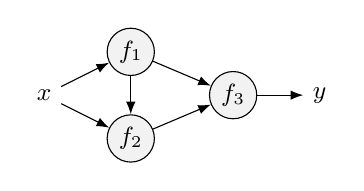
\begin{tikzpicture}[font=\small, >={Latex[length=1.6mm]},
  f/.style={draw, circle, fill=black!5, inner sep=1pt, minimum size=0.6cm}]
\node (x) at (0,0) {$x$};
\node[f] (f1) at (1.1,0.55) {$f_1$};
\node[f] (f2) at (1.1,-0.55) {$f_2$};
\node[f] (f3) at (2.4,0) {$f_3$};
\node (y) at (3.5,0) {$y$};
\draw[->] (x) -- (f1); \draw[->] (x) -- (f2);
\draw[->] (f1) -- (f2); \draw[->] (f1) -- (f3);
\draw[->] (f2) -- (f3); \draw[->] (f3) -- (y);
\end{tikzpicture}
\caption{Function network.}
\label{fig:fn}
\end{wrapfigure}
The search method treats the workflow as a function
network~\cite{astudillo2021} (Fig.~\ref{fig:fn}). Each step gets its own
statistical model, which predicts the outputs of that step together with
their uncertainty. The models are linked in the same order as the steps
(Fig.~\ref{fig:network}), so the outputs of one step are inputs to the next
and uncertainty propagates through the whole chain. We use a Gaussian process
for each node model for its predictive accuracy, well-calibrated uncertainty,
and gradients available through automatic differentiation. Because each step
has its own model, the network learns from partial results, and a candidate
can stop at any step. Buathong et al.\ added a cost-aware rule to this
network~\cite{buathong2024}. For each possible experiment, it estimates how
much the result is expected to improve the search, divides that by the
experiment's cost, and runs the best one, for a single property of interest
and one experiment at a time, and was shown only on simple networks. Our network combines simulations and experiments. The simulations
are calculations of phase diagrams (CALPHAD) in Thermo-Calc and
pycalphad~\cite{andersson2002,otis2017}, which give freezing range,
solidification phases, and a cracking index~\cite{kou2015}.

\begin{figure}[t]
\centering
\setstretch{1}  % diagram labels only; body and captions keep 1.5 spacing
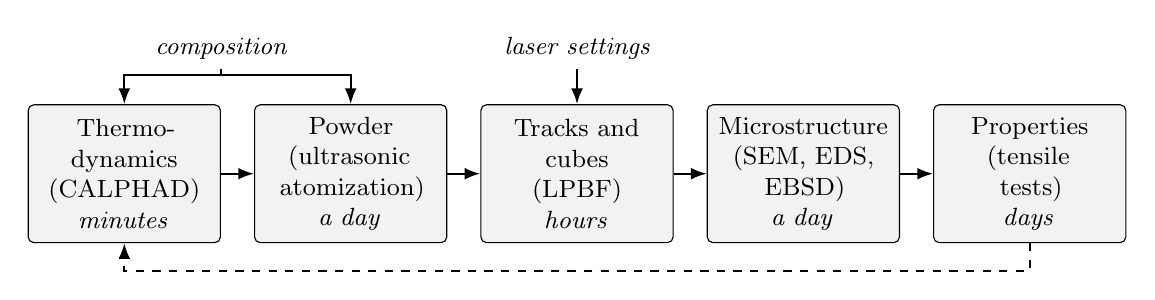
\begin{tikzpicture}[
  font=\small,
  node distance=0.42cm,
  box/.style={draw, rounded corners=2pt, fill=black!5, align=center,
    text width=2.3cm, minimum height=1.75cm, inner sep=2pt},
  arr/.style={-{Latex[length=2mm]}, thick},
  input/.style={font=\small\itshape, align=center}
]
\node[box] (s1) {Thermo-\\dynamics\\(CALPHAD)\\\textit{minutes}};
\node[box, right=of s1] (s2) {Powder\\(ultrasonic\\atomization)\\\textit{a day}};
\node[box, right=of s2] (s3) {Tracks and\\cubes\\(LPBF)\\\textit{hours}};
\node[box, right=of s3] (s4) {Microstructure\\(SEM, EDS,\\EBSD)\\\textit{a day}};
\node[box, right=of s4] (s5) {Properties\\(tensile\\tests)\\\textit{days}};
\foreach \a/\b in {s1/s2, s2/s3, s3/s4, s4/s5} \draw[arr] (\a) -- (\b);
\node[input, above=0.45cm of s1.north east] (comp) {composition};
\draw[arr] (comp.south) -- ++(0,-0.08) -| (s1.north);
\draw[arr] (comp.south) -- ++(0,-0.08) -| (s2.north);
\node[input, above=0.45cm of s3] (laser) {laser settings};
\draw[arr] (laser) -- (s3);
\draw[arr, dashed] (s5.south) -- ++(0,-0.35) -| (s1.south);
\end{tikzpicture}
\caption{The workflow as linked models (typical time per result in
italics). Dashed: results update the models, which pick the next step.}
\label{fig:network}
\end{figure}

\subsection{Method advances}
The published cost-aware network method has three limits that matter for
real experiments. First, it optimizes a
single objective. A printed aluminum alloy for aircraft parts must balance
freedom from cracks and pores, strength, and ductility, with no weighting
known in advance. We will
extend the cost-aware rule to several objectives. The expected improvement in
one objective will be replaced by the expected growth of the set of best
trade-offs (the Pareto front), measured by hypervolume as in multi-objective
Bayesian optimization~\cite{daulton2021}, and divided by cost as before. The
difficulty is that a cheap early measurement informs some objectives strongly
and others weakly. Single laser tracks, for example, show cracking well but
say little about strength, and the rule has to account for that through
the network.

Second, the method chooses one experiment at a time and waits for its result.
A build plate holds dozens of tracks and cubes, microscopy results arrive days
after printing, and thermodynamic calculations finish in minutes. We will
extend the rule to batches whose results arrive at different times, so that
new experiments are chosen while others are still pending, with the pending
ones accounted for in the models. We will also test how stable the choices are
when a late result contradicts early ones. This responds to the portfolio's
call for ``asynchronous algorithms'' with ``stable and robust convergence
properties under perturbations induced by time-dependent \ldots{} data
inputs.''

Third, published tests of these methods use test functions and
simulators~\cite{astudillo2021,buathong2024}. This project will demonstrate
them on a five-step physical workflow (Fig.~\ref{fig:network}), from making the powder to tensile
tests, with real build-to-build scatter,
outputs computed from microscopy images, and two inputs (composition and
laser settings) entering at different steps. CALPHAD outputs will also enter
the models as physics inputs, a test of physics-enhanced machine learning
where the physics is incomplete, since standard CALPHAD calculations ignore
the very fast cooling of the melt pool~\cite{debroy2018}.

To our knowledge, no multi-objective or asynchronous version of cost-aware,
partial-evaluation network optimization exists, and none has run on a
physical alloy workflow. Multi-stage Bayesian optimization was tested on
synthetic and retrospective data with one objective~\cite{torresi2026};
cost-aware batch optimization of refractory alloys treats unequal-cost
measurements as separate sources, not linked steps~\cite{alvi2026}; and
closed-loop printed-alloy campaigns use one model and fixed
measurements~\cite{talbot2026}.

\subsection{Hypotheses}
H1: the asynchronous, multi-objective, cost-aware network search will reach
a target set of trade-offs at lower total cost than standard batch
multi-objective Bayesian optimization that carries every candidate through
the full chain. H2: based on our preliminary results (Section~5), the
advantage will be largest when the physics at early steps misses a key
effect of the real experiments. H3: CALPHAD outputs used as physics inputs
will improve calibration of the predicted probability that a candidate is
dense and crack-free. A physical campaign
cannot be repeated often enough to test H1 and H2 statistically, so both
will be tested on many repeated campaigns over synthetic benchmarks and over
retrospective benchmarks built from our own data. H1 will be rejected if the
median cost to reach the target is not lower than the baseline's, H2 if the
advantage is not larger with a physics gap than without, and H3 if physics
inputs do not reduce calibration error on held-out live builds.

\subsection{Approach, data, and analysis}
\begin{figure}[t]
\centering
\begin{minipage}[c]{3.75in}
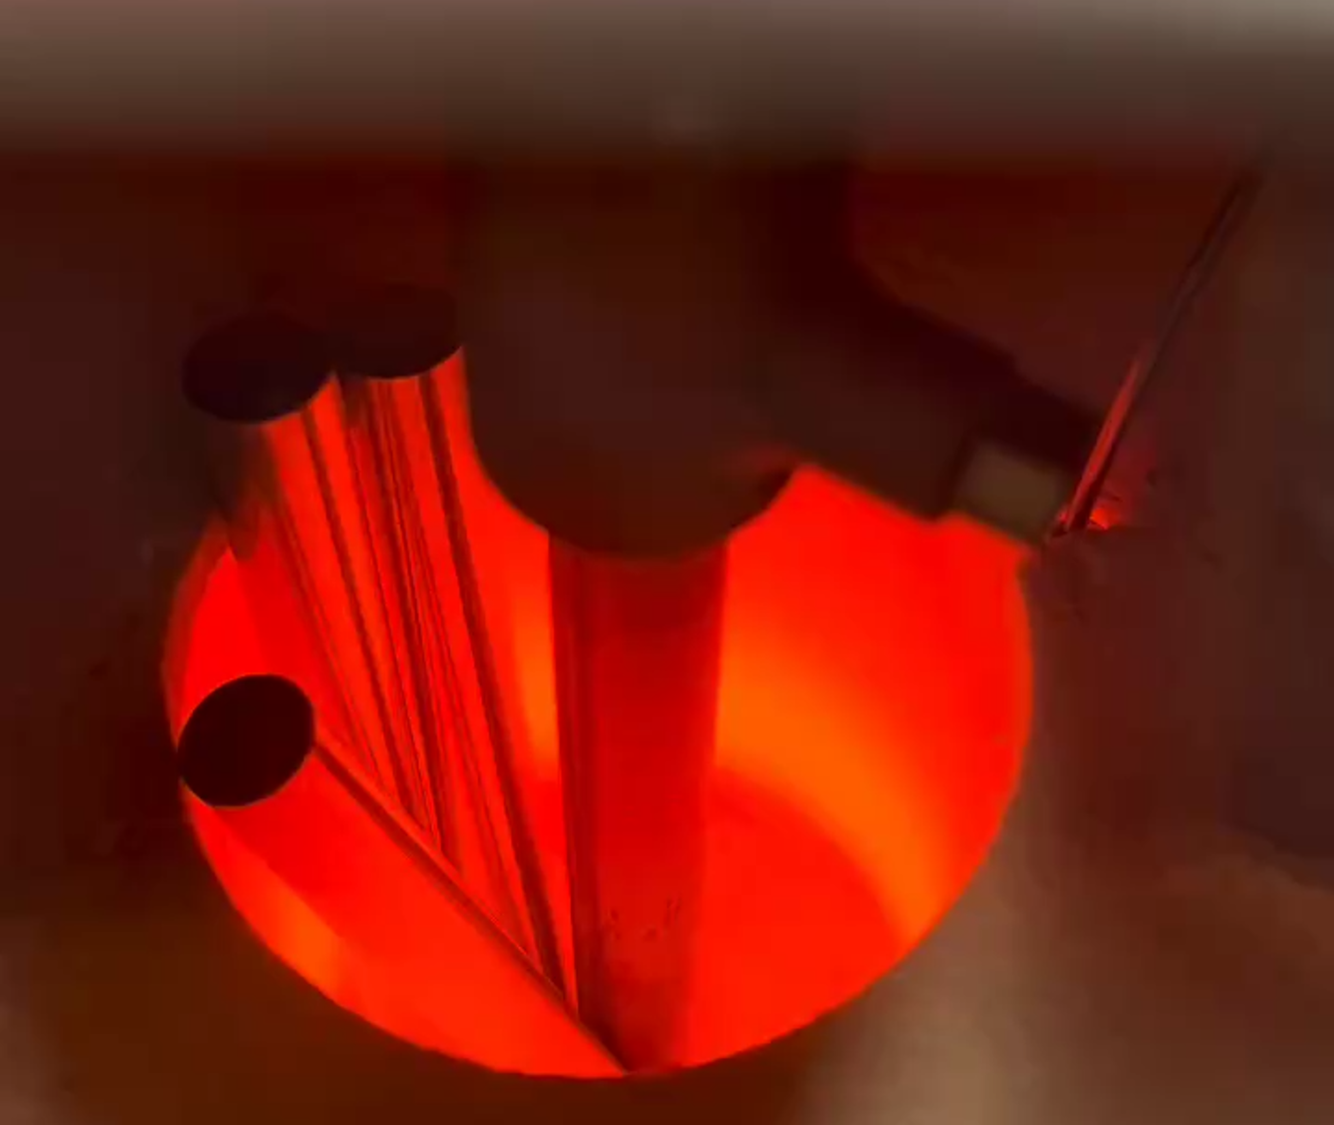
\includegraphics[height=0.95in]{../figures/al-melting-rods.png}\hfill
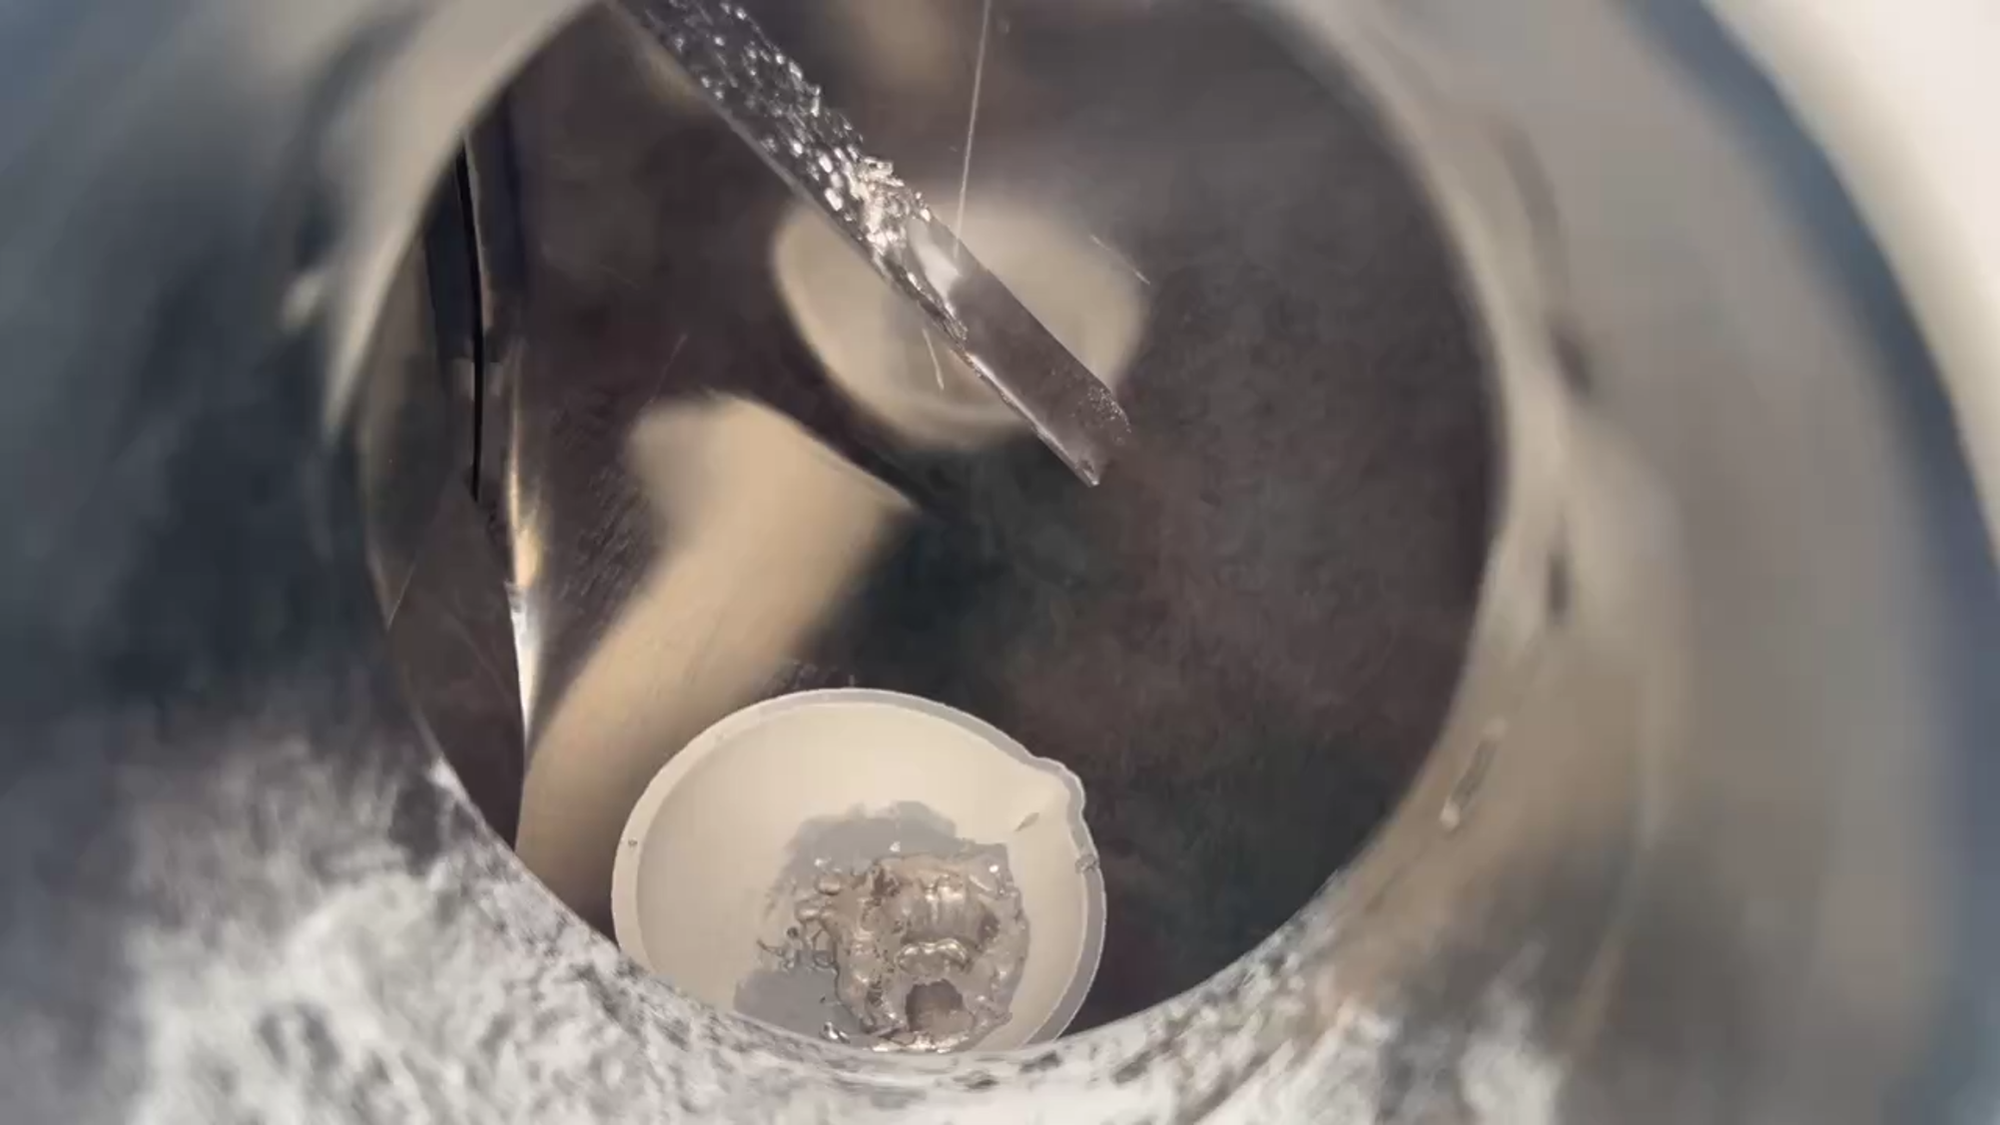
\includegraphics[height=0.95in]{../figures/al-melt-stream.png}\hfill
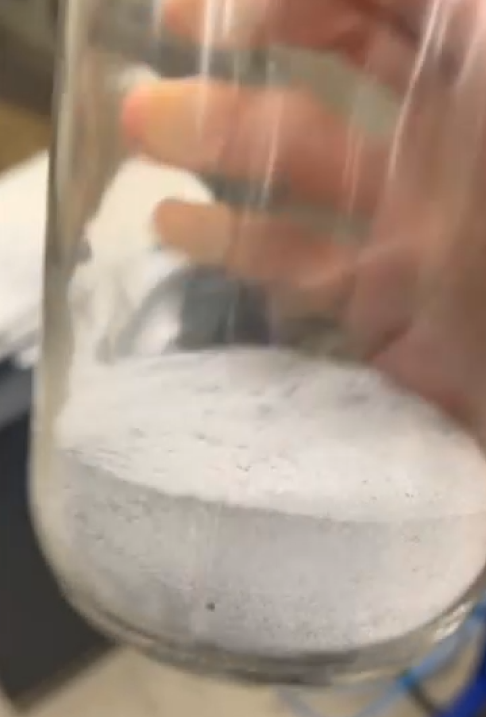
\includegraphics[height=0.95in]{../figures/our-atomized-powder.png}
\end{minipage}\hfill
\begin{minipage}[c]{2.65in}
\caption{In our atomizer: aluminum rods melting, the melt stream on the
plate, and our powder.}
\label{fig:atomizer}
\end{minipage}
\end{figure}
Powder for each candidate will be made in our laboratory (Fig.~\ref{fig:atomizer}) by an ultrasonic
atomizer (AMAZEMET rePOWDER) whose induction-melting module covers aluminum
alloys and makes four compositions per week. Each round, the platform will choose compositions and laser settings (power,
scan speed, and hatch spacing). Single laser tracks show melt-pool size,
balling, and cracking, and small cubes give density and porosity. Selected
cubes will be examined by scanning electron microscopy (SEM), by
energy-dispersive X-ray spectroscopy (EDS) for composition, since magnesium
and zinc can evaporate during melting~\cite{debroy2018}, and by electron
backscatter diffraction (EBSD) for grain size and shape. The most promising
candidates will get tensile tests, with hardness as a cheaper stand-in.
Replicate tracks and cubes at fixed settings will measure build-to-build
scatter. Baselines are random selection and full-chain batch multi-objective
Bayesian optimization at equal budgets, with benchmarks fixed before
campaigns start. Data, code,
and models will be made publicly available, and results that reject a hypothesis
will be published like any other result, per Gold Standard Science
(NOFO Section C.3).

\section{Potential team members and development plan}

The PI will lead method development and supervise one Ph.D. student,
funded for three years, who will run the LPBF and characterization campaigns,
and two part-time undergraduate researchers, who will make powder
and prepare specimens. LPBF builds will be bought from a University of Utah user facility at
\$800 per build. All other work will be at BYU: the PI's atomizer laboratory,
the Microscopy Center (SEM, EDS, EBSD), and
high-performance computing.

Year~1 will develop the asynchronous and multi-objective extensions, build
synthetic and retrospective benchmarks from the aluminum data in hand, and
measure scatter with replicated tracks and cubes. Year~2 will test H1 and H2
on the benchmarks and run live campaigns with EBSD and tensile tests. Year~3 will test H3 on held-out live builds and
release the software and data.

\section{Preliminary results and PI qualifications}

Since December 2025, we have set up a CALPHAD workflow on BYU high-performance computing and tested each step of the proposed workflow on its own: atomized powder,
LPBF builds, SEM and EDS, and tensile tests, de-risking the workflow.

% Fig. 3 redraws the synthetic network from the MS&T26 talk
% (benchmarks/bofn-prelim/explain/frames/00-network.png) as a short strip;
% node functions and costs are in benchmarks/bofn-prelim/README.md.
\begin{figure}[t]
\centering
\setstretch{1}  % diagram labels only; body and captions keep 1.5 spacing
\resizebox{\textwidth}{!}{%
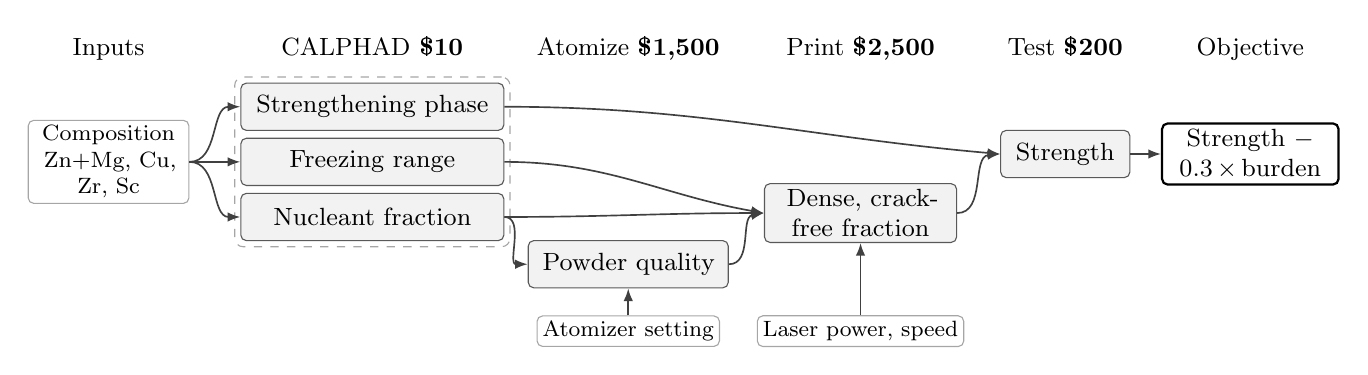
\begin{tikzpicture}[
  font=\small,
  nd/.style={draw=black!65, rounded corners=2pt, fill=black!5, align=center,
    minimum height=0.6cm, inner sep=2pt},
  inp/.style={draw=black!35, rounded corners=2pt, align=center,
    font=\footnotesize, inner sep=2pt},
  hd/.style={font=\small, anchor=base},
  e/.style={-{Latex[length=1.6mm]}, black!75, semithick}
]
\foreach \x/\t in {0.95/Inputs, 4.3/{CALPHAD \textbf{\$10}},
  7.55/{Atomize \textbf{\$1,500}}, 10.5/{Print \textbf{\$2,500}},
  13.1/{Test \textbf{\$200}}, 15.45/Objective}
  \node[hd] at (\x,2.75) {\t};
\node[inp, text width=1.9cm] (c) at (0.95,1.4) {Composition\\Zn+Mg, Cu,\\Zr, Sc};
\node[nd, text width=3.2cm] (s) at (4.3,2.1) {Strengthening phase};
\node[nd, text width=3.2cm] (f) at (4.3,1.4) {Freezing range};
\node[nd, text width=3.2cm] (g) at (4.3,0.7) {Nucleant fraction};
\node[draw=black!35, dashed, rounded corners=3pt, inner sep=2pt,
  fit=(s)(f)(g)] {};
\node[nd, text width=2.4cm] (q) at (7.55,0.1) {Powder quality};
\node[nd, text width=2.3cm] (r) at (10.5,0.75) {Dense, crack-\\free fraction};
\node[nd, text width=1.5cm] (u) at (13.1,1.5) {Strength};
\node[nd, draw=black, thick, fill=white, text width=2.1cm] (o) at (15.45,1.5)
  {Strength $-$\\0.3\,$\times$\,burden};
\node[inp] (a) at (7.55,-0.75) {Atomizer setting};
\node[inp] (l) at (10.5,-0.75) {Laser power, speed};
\foreach \n in {s,f,g} \draw[e] (c.east) to[out=0, in=180] (\n.west);
\draw[e] (s.east) to[out=0, in=175] (u.west);
\draw[e] (f.east) to[out=0, in=170] (r.west);
\draw[e] (g.east) to[out=0, in=180] (r.west);
\draw[e] (g.east) to[out=0, in=180] (q.west);
\draw[e] (q.east) to[out=0, in=190] (r.west);
\draw[e] (r.east) to[out=0, in=185] (u.west);
\draw[e] (u) -- (o);
\draw[e] (a) -- (q);
\draw[e] (l) -- (r);
\end{tikzpicture}}
\caption{Synthetic network for Fig.~\ref{fig:sim}, with rough total cost per
step. Nucleant (Zr, Sc) cuts cracking unseen by CALPHAD.}
\label{fig:synth}
\end{figure}


\begin{wrapfigure}{r}{2.7in}
\vspace{-12pt}
\centering
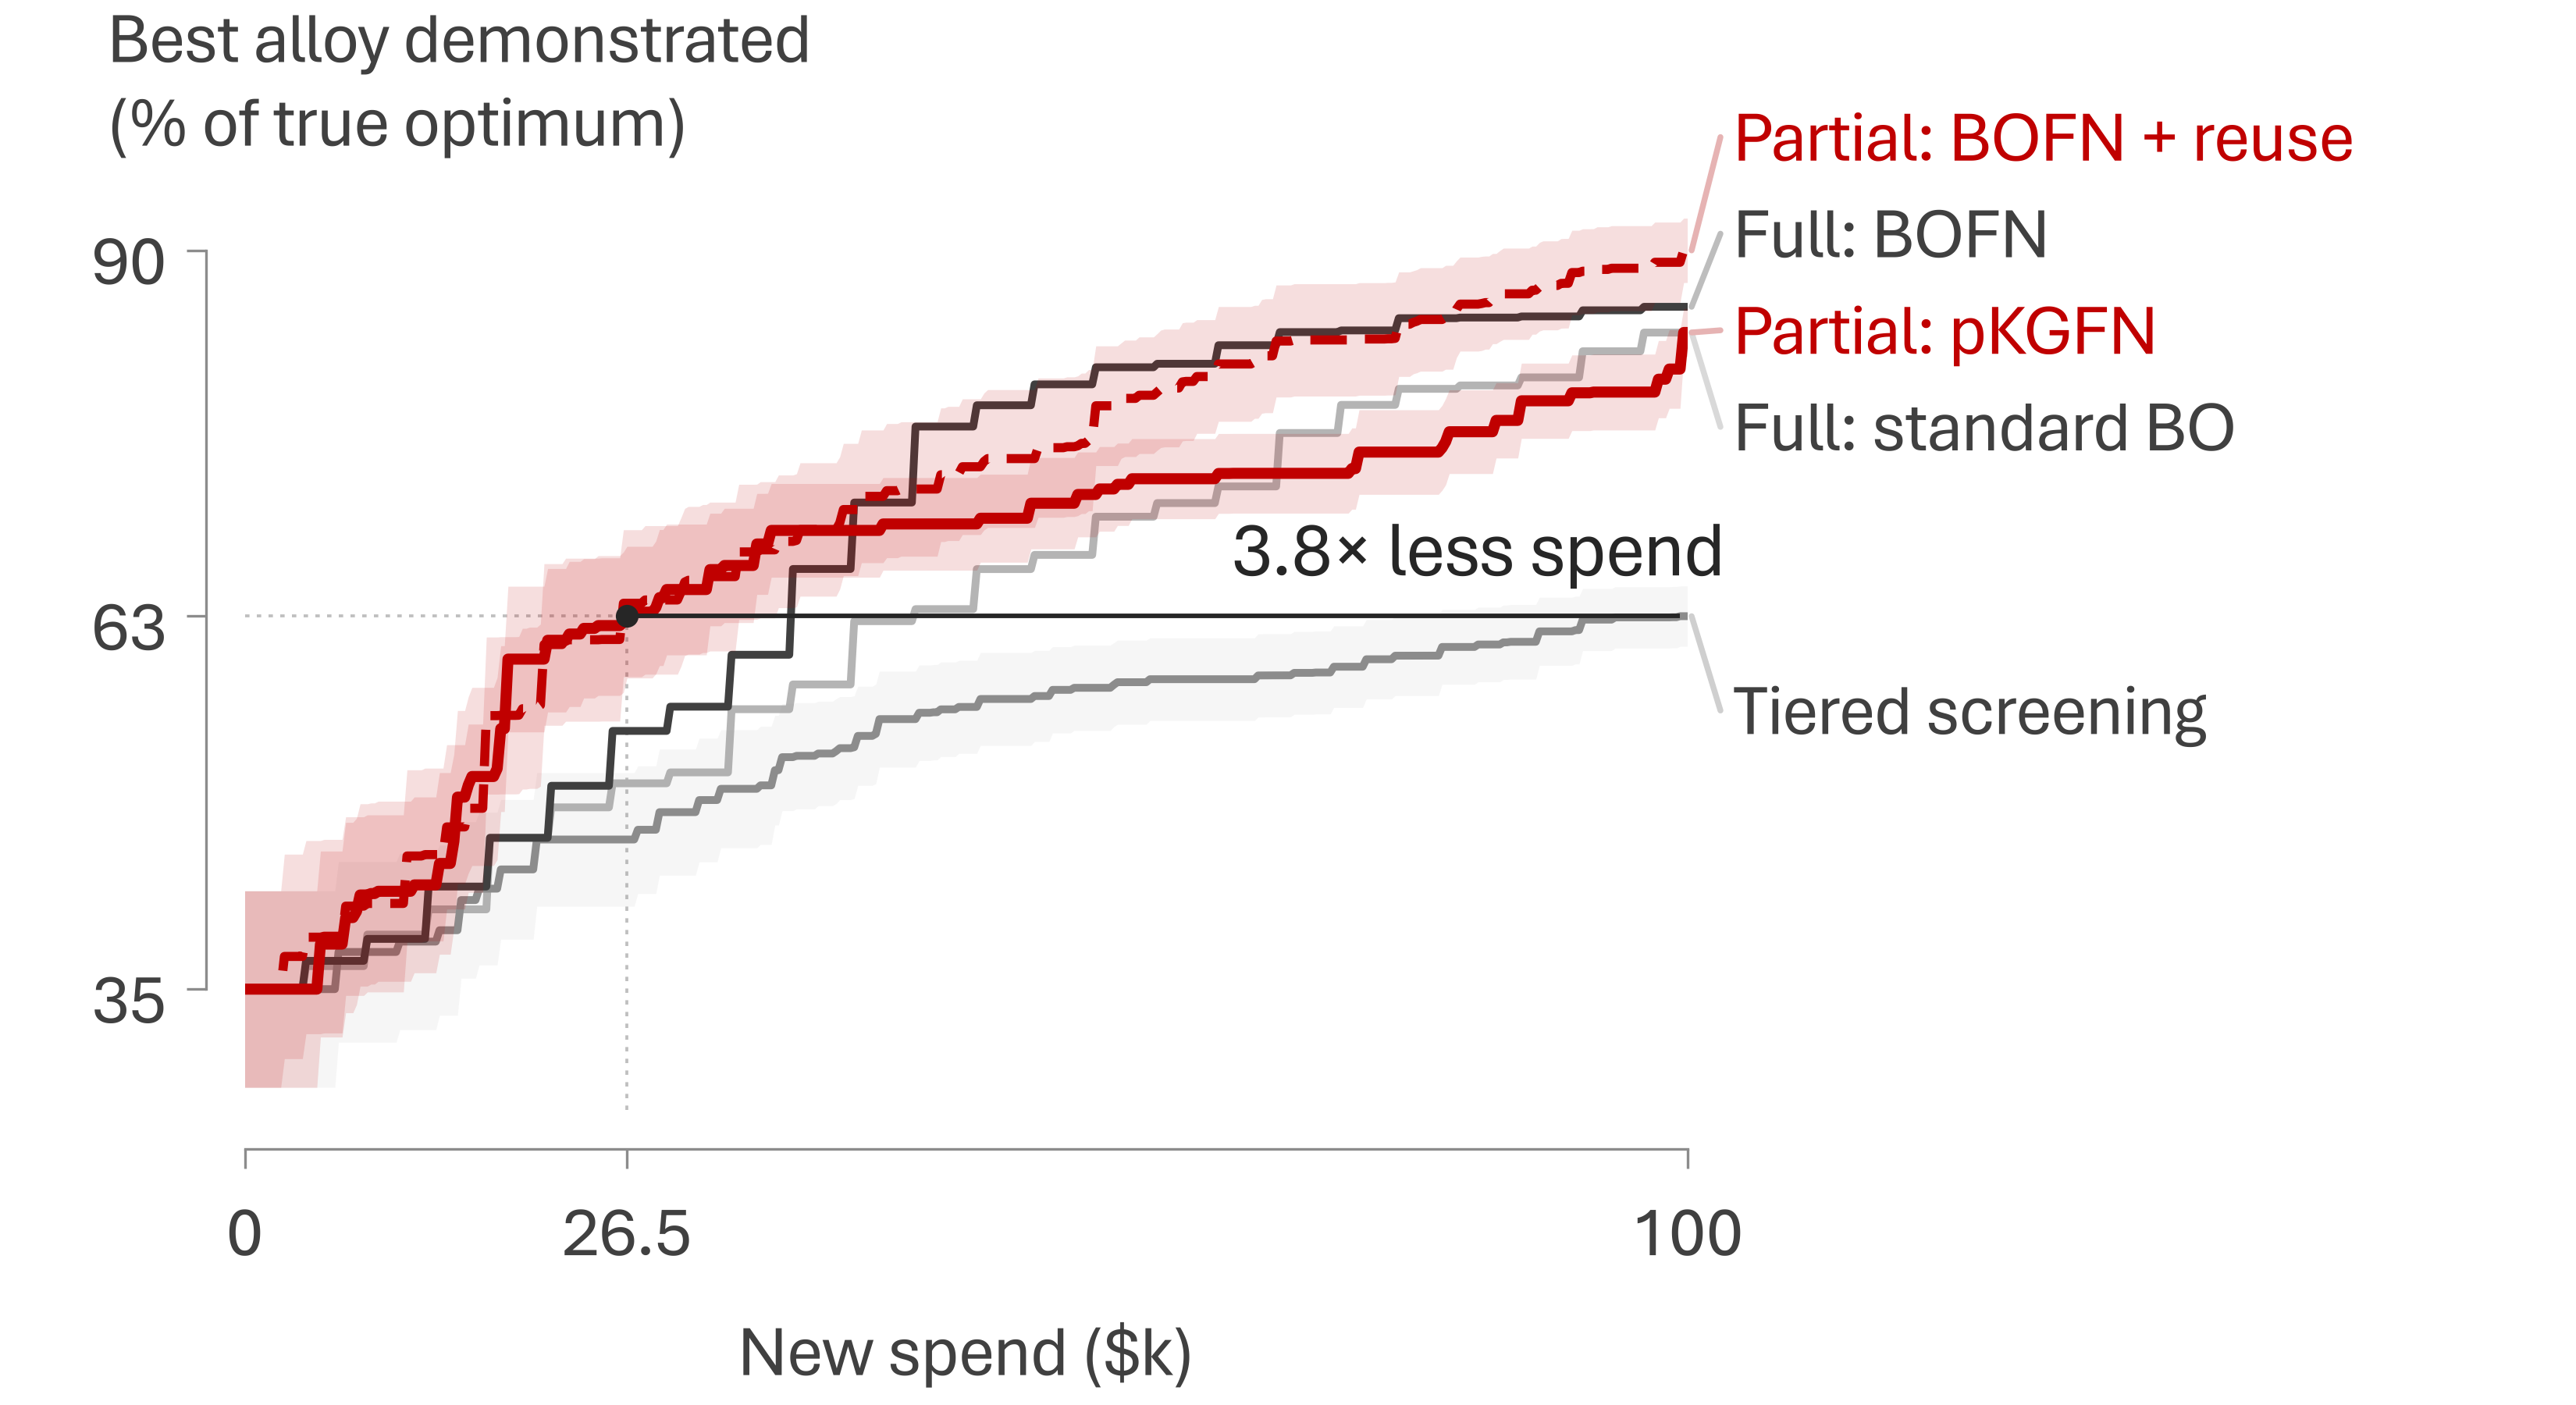
\includegraphics[width=\linewidth]{../benchmarks/bofn-prelim/bofn_best_vs_spend_k1_partial_vs_full.png}
\caption{Crack screen ignores Zr (mean of 20,
$\pm$1 s.e.). Red: search picks the next step; gray: fixed order.}
\label{fig:sim}
\vspace{-8pt}
\end{wrapfigure}
We also simulated the cost-aware network method on a
synthetic version of the workflow (Figs.~\ref{fig:synth} and~\ref{fig:sim}). With the crack screen ignoring zirconium, screening and
then tuning the process stalled at 63\% of the optimum after \$100,000. The
cost-aware search, and a simpler one that reused powders, reached that level
after about \$26,500 (3.8 times less spend; 90\% CI 2.0 to 5.7). Full-chain
searches caught up later, and screening kept pace when its physics was right.
The simulation is hand-built and noise-free, with one objective and one
experiment at a time, so it does not test the advances above. It supports H2: partial
evaluation matters most when simulations miss key features of real
experiments, as is likely where thermodynamic databases are sparse, in
less-explored compositions.

The PI developed Honegumi for setting up Bayesian optimization, consulted on
Meta's Ax 1.0, co-authored the \emph{Chemical Reviews} survey of self-driving
laboratories, and built the Acceleration Consortium's development laboratory
at the University of Toronto. He has 11 first-author peer-reviewed journal
articles (23 in all; see CV).

% ===========================================================================
% References (excluded from the 5-page limit)
% ===========================================================================
\clearpage
\setcounter{page}{1}
\renewcommand{\thepage}{R\arabic{page}}  % keep reference pages out of 1-5
\begin{thebibliography}{99}
\setlength{\itemsep}{2pt}

\bibitem{martin2017}
J.~H. Martin, B.~D. Yahata, J.~M. Hundley, J.~A. Mayer, T.~A. Schaedler, and
T.~M. Pollock, ``3D printing of high-strength aluminium alloys,''
\emph{Nature} \textbf{549}, 365--369 (2017).
\href{https://doi.org/10.1038/nature23894}{doi:10.1038/nature23894}

\bibitem{debroy2018}
T.~DebRoy, H.~L. Wei, J.~S. Zuback, T.~Mukherjee, J.~W. Elmer,
J.~O. Milewski, A.~M. Beese, A.~Wilson-Heid, A.~De, and W.~Zhang, ``Additive
manufacturing of metallic components -- Process, structure and properties,''
\emph{Prog. Mater. Sci.} \textbf{92}, 112--224 (2018).
\href{https://doi.org/10.1016/j.pmatsci.2017.10.001}{doi:10.1016/j.pmatsci.2017.10.001}

\bibitem{baa2026}
AFOSR BAA FA955026S0001, Amendment 0001 (21 Aug 2026), Section A.2.c,
Dynamic Data and Information Processing. See also F.~Darema, E.~P. Blasch,
S.~Ravela, and A.~J. Aved (eds.), \emph{Handbook of Dynamic Data Driven
Applications Systems}, Vol.~2 (Springer, 2023).
\href{https://doi.org/10.1007/978-3-031-27986-7}{doi:10.1007/978-3-031-27986-7}

\bibitem{dursun2014}
T.~Dursun and C.~Soutis, ``Recent developments in advanced aircraft aluminium
alloys,'' \emph{Mater. Des.} \textbf{56}, 862--871 (2014).
\href{https://doi.org/10.1016/j.matdes.2013.12.002}{doi:10.1016/j.matdes.2013.12.002}

\bibitem{dodig2019}
Inspector General, U.S. Department of Defense, \emph{Audit of the DoD's Use of
Additive Manufacturing for Sustainment Parts}, Report No.~DODIG-2020-003
(17 Oct 2019).
\href{https://media.defense.gov/2019/Oct/21/2002197659/-1/-1/1/DODIG-2020-003.PDF}{media.defense.gov/2019/Oct/21/2002197659}

\bibitem{campo2026}
E.~M. Campo, R.~J. Hanisch, and J.~C. Agar, ``From discovery to deployment:
A national AI strategy for materials readiness across energy and defense,''
\emph{MRS Bull.} (2026), published online 23 Sep 2026.
\href{https://doi.org/10.1557/s43577-026-01181-0}{doi:10.1557/s43577-026-01181-0}

\bibitem{astudillo2021}
R.~Astudillo and P.~I. Frazier, ``Bayesian optimization of function networks,''
\emph{Advances in Neural Information Processing Systems} \textbf{34},
14463--14475 (2021).
\href{https://proceedings.neurips.cc/paper_files/paper/2021/hash/792c7b5aae4a79e78aaeda80516ae2ac-Abstract.html}{NeurIPS proceedings},
\href{https://arxiv.org/abs/2112.15311}{arXiv:2112.15311}

\bibitem{buathong2024}
P.~Buathong, J.~Wan, R.~Astudillo, S.~Daulton, M.~Balandat, and P.~I. Frazier,
``Bayesian optimization of function networks with partial evaluations,''
\emph{Proc. 41st Int. Conf. Machine Learning (ICML)}, PMLR \textbf{235},
4752--4784 (2024).
\href{https://proceedings.mlr.press/v235/buathong24a.html}{PMLR proceedings},
\href{https://arxiv.org/abs/2311.02146}{arXiv:2311.02146}

\bibitem{andersson2002}
J.-O. Andersson, T.~Helander, L.~H{\"o}glund, P.~Shi, and B.~Sundman,
``Thermo-Calc \& DICTRA, computational tools for materials science,''
\emph{Calphad} \textbf{26}(2), 273--312 (2002).
\href{https://doi.org/10.1016/S0364-5916(02)00037-8}{doi:10.1016/S0364-5916(02)00037-8}

\bibitem{otis2017}
R.~Otis and Z.-K. Liu, ``pycalphad: CALPHAD-based computational thermodynamics
in Python,'' \emph{J. Open Res. Softw.} \textbf{5}(1), 1 (2017).
\href{https://doi.org/10.5334/jors.140}{doi:10.5334/jors.140}

\bibitem{kou2015}
S.~Kou, ``A criterion for cracking during solidification,''
\emph{Acta Mater.} \textbf{88}, 366--374 (2015).
\href{https://doi.org/10.1016/j.actamat.2015.01.034}{doi:10.1016/j.actamat.2015.01.034}

\bibitem{daulton2021}
S.~Daulton, M.~Balandat, and E.~Bakshy, ``Parallel Bayesian optimization of
multiple noisy objectives with expected hypervolume improvement,''
\emph{Advances in Neural Information Processing Systems} \textbf{34} (2021).
\href{https://arxiv.org/abs/2105.08195}{arXiv:2105.08195}

\bibitem{torresi2026}
L.~Torresi and P.~Friederich, ``Multi-stage Bayesian optimisation for dynamic
decision-making in self-driving labs,'' \emph{Digital Discovery} \textbf{5},
1900--1912 (2026).
\href{https://doi.org/10.1039/d5dd00572h}{doi:10.1039/d5dd00572h}

\bibitem{alvi2026}
S.~M.~A.~A. Alvi, B.~Vela, V.~Attari, J.~Janssen, D.~Perez, D.~Allaire, and
R.~Arr{\'o}yave, ``Deep Gaussian process-based cost-aware batch Bayesian
optimization for complex materials design campaigns,''
\emph{npj Comput. Mater.} \textbf{12}, 105 (2026).
\href{https://doi.org/10.1038/s41524-026-01981-7}{doi:10.1038/s41524-026-01981-7}

\bibitem{talbot2026}
A.~Talbot, S.~S. Dash, J.~Li, C.~Cheng, M.~Ramesh, X.~Shang, J.~Zhang,
C.~Cojocaru, J.~Hattrick-Simpers, and Y.~Zou, ``Active learning for the
accelerated discovery of complex concentrated NiCoCr alloys in additive
manufacturing,'' \emph{npj Adv. Manuf.} (2026), published online 23 Jun 2026.
\href{https://doi.org/10.1038/s44334-026-00098-5}{doi:10.1038/s44334-026-00098-5}

\end{thebibliography}

% ===========================================================================
% Curriculum vitae (excluded from the 5-page limit; NOFO: "All publications
% and presentations must be identified")
% ===========================================================================
\IfFileExists{../bios/baird-CV.pdf}{%
  \includepdf[pages=-,pagecommand={\thispagestyle{empty}}]{../bios/baird-CV.pdf}%
}{}

\end{document}
